\subsection{Diagonalization and Power Sets}

\begin{theorem} \label{thm:cantor-power-set-theorem} \hlt{Cantor's Theorem}\\
Let $X$ be a set. No map $f:X\to\mathcal{P}(X)$ is surjective. Hence $X\not\sim_{\#}\mathcal{P}(X)$.
\begin{proof} Fix $f:X\to\mathcal{P}(X)$ and set $D_f\defeq\{x\in X:x\notin f(x)\}$.\\
If $f$ were surjective, then $D_f=f(a)$ for some $a\in X$. Hence $a\in D_f\Longleftrightarrow a\notin f(a)\Longleftrightarrow a\notin D_f$, a contradiction.\\
Thus no $f:X\to\mathcal{P}(X)$ is surjective, so no bijection $X\to\mathcal{P}(X)$ exists.\\
\hlt{Structural Commentary}: The diagonal subset escapes $f$.\\
\hlt{Key Insight}: Flip membership at $x$.
\end{proof}
\end{theorem}

\begin{figure}[H]
  \centering
  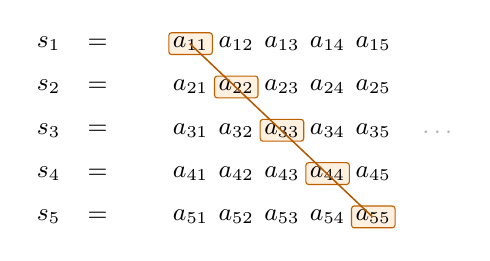
\begin{tikzpicture}[
  every node/.style={font=\small},
  digit/.style={font=\small},
  diagonal/.style={draw=orange!75!black, fill=orange!12, rounded corners=1pt, inner sep=1.5pt},
  guide/.style={orange!70!black, line width=0.55pt}
]
  \foreach \row/\name in {1/s_1,2/s_2,3/s_3,4/s_4,5/s_5} {
    \node[anchor=east] at (0,-0.55*\row) {$\name$};
    \node at (0.35,-0.55*\row) {$=$};
  }

  \foreach \row in {1,...,5} {
    \foreach \col in {1,...,5} {
      \node[digit] at (0.95+0.58*\col,-0.55*\row) {$a_{\row\col}$};
    }
  }

  \foreach \row in {1,...,5} {
    \node[diagonal] at (0.95+0.58*\row,-0.55*\row) {$a_{\row\row}$};
  }
  \draw[guide] (1.52,-0.55) -- (3.84,-2.75);

  \node[anchor=west, gray!60] at (4.35,-1.68) {$\cdots$};
\end{tikzpicture}

  \caption{Cantor diagonalization: $s(n)=1-a_{nn}$ differs from row $s_n$ at position $n$.}
  \label{fig:cantor-diagonal-binary-sequences}
\end{figure}

\begin{theorem} \label{thm:binary-sequences-uncountable} \hlt{Binary Sequences Are Uncountable}\\
Let $A$ be the set of all sequences whose terms are the digits $0$ and $1$. Then $A$ is uncountable.
\begin{proof}
Suppose $A$ were countable, $A=\{s_1,s_2,\ldots\}$ with $s_n=(s_n(k))_{k\in\N}$. Define $s\in A$ by $s(k)\defeq 1-s_k(k)$.\\
Then $s(n)\neq s_n(n)$ for every $n$, so $s\neq s_n$ for all $n$. Hence $s\notin A$, a contradiction. Thus $A$ is uncountable.\\
\hlt{Structural Commentary}: The construction attacks the diagonal of a proposed enumeration.\\
\hlt{Key Insight}: A sequence can be built to escape every row of a countable list.
\end{proof}
\end{theorem}

\begin{definition} \label{def:continuum-cardinal} \hlt{Continuum Cardinal}\\
The \hlt{continuum cardinal} is $\mathfrak{c}\defeq 2^{\aleph_0}\defeq\abs{\{0,1\}^{\N}}$. Equivalently, $\mathfrak{c}=\abs{\mathcal{P}(\N)}$ via $s\mapsto\{n\in\N:s(n)=1\}$.
\end{definition}

\begin{perspective} \label{per:continuum-and-powerset-cardinality} \hlt{Continuum Cardinality}\\
Theorem \ref{thm:binary-sequences-uncountable} and Theorem \ref{thm:cantor-power-set-theorem} give $\aleph_0<\mathfrak{c}$.\\
Thus the continuum is the first cardinal jump produced by binary choice over $\N$.
\end{perspective}
